\section{Ridge Mapping}
\label{sec:ridge-mapping}

Given a function, $E$, of multiple variables, $\vR$, its gradient, $\nabla E(\vR)$, and two \sap{1}s, the goal is to identify a path that lies close to the ridge between the \sap{1}s.
The path should, in particular, lie through any intermediate \sap{2}s so that a comparison of their height with respect to the endpoints can be made.
The method should, furthermore, lead to the identification of previously unknown \sap{1}(s) on the ridge in between the given end points, should they exist.

\subsubsection{Gradient Modification}
\begin{SCfigure}[5.0][h]
%\begin{center}
\centering
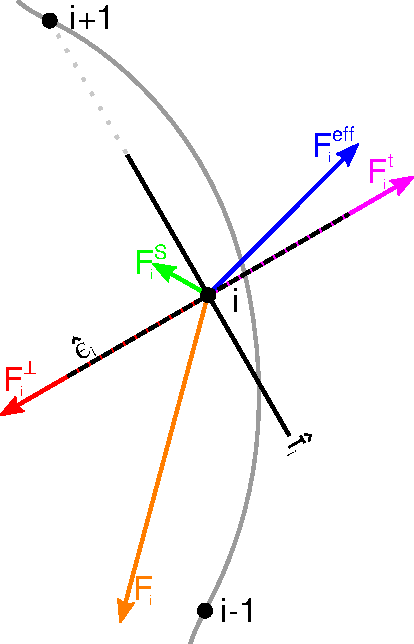
\includegraphics[width = 0.35\linewidth]{erm-forces}
%    \parbox{0.85\linewidth}{
\caption{
The construction of the effective force, $\vF^\text{eff}_i$,
which acts on image $i$ (the label, $i$, is excluded from all the force symbols) of the path and is used in the iterative optimisation.
The solid grey line indicates the ridge,
the black filled circles represent the current location of three adjacent images,
the black solid line shows the tangent estimate, $\uvt_i$
and the black dashed line shows the minimum mode estimate, $\uvn_i$.
The orange arrow shows the gradient force, $\vF_i= -\nabla E$.
The red arrow shows the transformed force, $\vF^t$ (\fref{eq:transformed-force}),
%obtained by inverting $\vF$ in the direction of the minimum mode, $\epsilon$ (see \eref{eq:minmode-force}).
The purple arrow shows $\vF_i^\perp$, the component of the transformed force that is perpendicular to the tangent.
The green arrow shows $\vF_i^\text{S}$ (\fref{eq:full-spring-force}), %the spring force given by \eref{eq:full-spring-force}.
The blue arrow shows $\vF_i^\text{eff}$ (\fref{eq:erm-effective-force}).
}
\label{fig:erm-forces}
%}
%\end{center}
\end{SCfigure}

Similarly to the NEB method~\cite{neb-original-1998} (\fref{sec:neb}), a path of $N$ discrete images, $[\vR_0, \vR_1, \ldots, \vR_N]$, is iteratively aligned with the ridge by modifying the gradient or force, $\vF_i \equiv -\nabla E(\vR_i)$, for each one.
However, unlike the NEB method, further force modifications are needed, in order to let the ridge appear as a MEP.

The path is at each image defined by its tangent, $\uvt_i$, and in order for the path to be at a SDP (such as the ridge), any force components perpendicular to it,
\beq{perpendicular-force}
\vF_i^\perp \equiv \vF_i -(\vF_i \cdot \uvt_i)\uvt_i,
\eeq
must be zero,
\beq{ridge-force}
\vF^\perp_\text{ridge} = \vect{0}.
\eeq
Furthermore, one negative eigenvalue of the Hessian, perpendicular to the path, must be guaranteed.\footnote{If finding higher order ridges is desired, more negative eigenvalues must be guaranteed.}
The Dimer methodology~\cite{dimer-original-1999, dimer-olsen-2004} (\fref{sec:dimer}) for finding the lowest eigenvalue and the corresponding eigenvector (minimum mode) of the Hessian, $\uvn_i$, can produce a transformed force,
\beq{transformed-force}
\vF_i^\text{t} = \vF_i^\perp - 2(\vF_i^\perp \cdot \uvn_i)\uvn_i,
\eeq
that will map convex degrees of freedom to concave ones, effectively making the ridge appear as a MEP with regards to the gradient.
Since eigenvectors are not necessarily perpendicular to the ridge (as can be seen in figure 1 of paper \ref{pap:second-order}), the path itself must be left out of the Hessian's vector space, thus applying an orthogonality constraint on the minimum mode,
\beq{orthogonality-constraint}
\uvt_i \cdot \uvn_i = 0,
\eeq
at all times.

Similarly to the NEB method, an artificial force is employed in order to keep the images equally\footnote{or with controlled spacing} distributed along the path.
For the NEB method this force acts only along the path and is generally referred to as the spring force as it resembles springs connecting the images.
However, in the case of ridge calculations, the full spring force must be used,
\beq{full-spring-force}
\vF_i^\text{S} = k \left[ \left( \vR_{i+1} - \vR_i \right) - \left( \vR_i - \vR_{i-1} \right) \right],
\eeq
where $k$ is the spring constant, which controls the stiffness of the springs.
Retention of the full spring force is necessary due to numerical instabilities which proved to be more prominent in ridge calculations than MEP calculations (see below).

Combining the above forces, $\vF_i^\text{t}$ and $\vF_i^\text{S}$, into an effective force (as shown in \fref{fig:erm-forces}),
\beq{erm-effective-force}
\vF_i^\text{eff} = \vF_i^\text{t} + \vF_i^\text{S},
\eeq
will allow the path iteratively converge close to the ridge.

\subsubsection{Exact Convergence to the \sap{2}}
Beyond the problems already discussed regarding converging exactly to the \sap{1} in NEB calculations, systematic errors due to the retention of the full spring force makes it unlikely that using only \fref{eq:erm-effective-force} will yield an image at the exact \sap{2}.
As with the NEB method a Dimer-type solution is possible --- similar to equations \ref{eq:dimer-transform} and \ref{eq:neb-ci-transform} --- where the highest value image is decoupled from the springs, forming the so-called climbing image, and force components along the \emph{two} lowest eigenvalued eigenmodes, as defined by the minimum mode and the tangent,
\beq{erm-ci}
\vF_{i_\text{max.}}^\text{eff.} = \vF_{i_\text{max.}} - 2(\vF_{i_\text{max.}} \cdot \uvt_{i_\text{max.}})\uvt_{i_\text{max.}} - 2(\vF_{i_\text{max.}} \cdot \uvn_{i_\text{max.}})\uvn_{i_\text{max}},
\eeq
where $i_\text{max.}$ refers to the image with the highest functional value.

Unlike the NEB, the computational effort involved is not easily measured due to the systematic errors introduced by the full spring force but there is no reason to suspect increased effort by applying \fref{eq:erm-ci}.
Furthermore, this addition can not be considered optional, as it can technically for NEB, since it serves as an indirect stabilisation tool at the top of the path, where the environment is concave\footnote{Curves downwards} in 2 dimensions rather than 1 as is the case with a MEP.

\subsection{Numerical Instabilities}

\subsubsection{The Orthogonality Constraint}
\begin{figure}[htb!]
\begin{center}
  \subfigure[The minimum mode is kept orthogonal to a central difference tangent.]{
    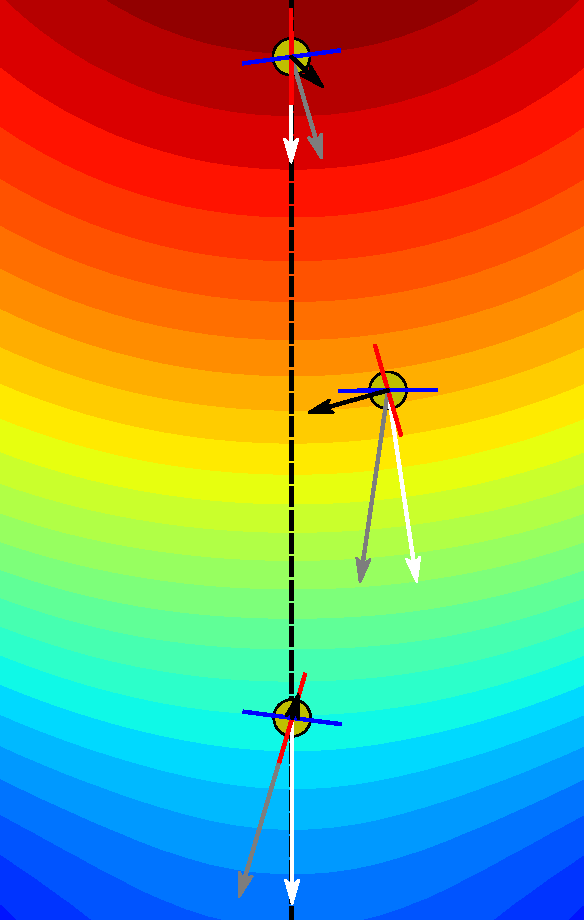
\includegraphics[width=0.45\linewidth]{orthogonal-good}
    \label{fig:orthogonal-good}
    }
  \subfigure[The minimum mode is kept orthogonal to the higher-image tangent.]{
    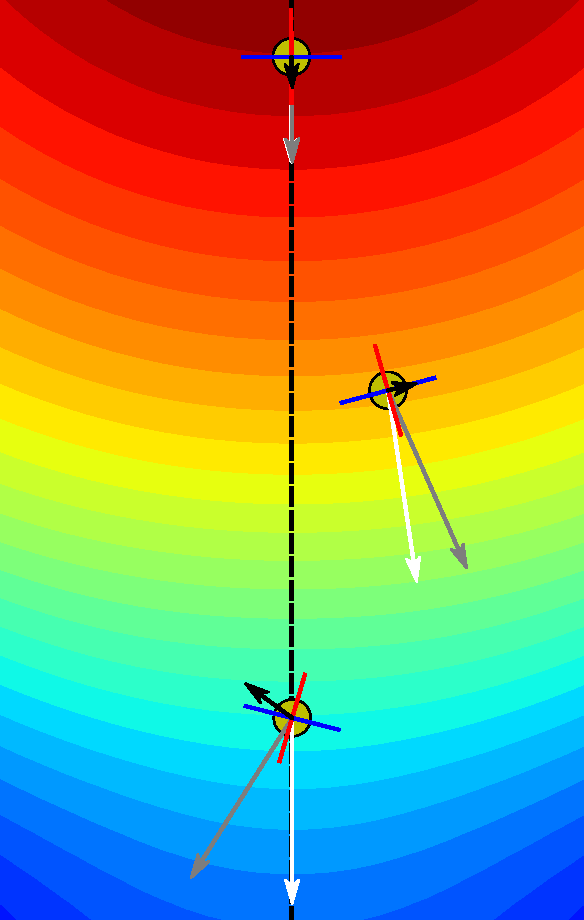
\includegraphics[width=0.45\linewidth]{orthogonal-bad}
    \label{fig:orthogonal-bad}
    }
    \parbox{0.85\linewidth}{
\caption{
The ridge is the black dashed line.
The white arrows are the PES force, the grey arrows are the dimer transformed forces and the black arrows are the effective forces.
The red line is the higher-image tangent and the blue line is the minimum mode estimate.
The system is a frozen 1 layer \ce{Al}(100) "slab" with a free to move \ce{Al} adatom, modelled with EMT~\cite{emt-1996} and the ridge is that between two neighbouring hop \sap{1}s.
The PES is created by relaxing the adatom in the direction perpendicular to the frozen layer.
Shown are the in-plane components of the forces and vectors.
The out-of-plane components for all are very small.
}
\label{fig:orthogonal}
}
\end{center}
\end{figure}

Simply using the Dimer, or any other non-exact, estimate of the minimum mode introduces instabilities in the forces, as the ridge$\rightarrow$MEP mapping can get inaccurate.
This is not a problem hindering convergence, directly, since the Dimer generally has ample time to converge to the nearly exact minimum mode during the iterative convergence.

More serious, seems to be the interaction between the minimum mode and the tangent, as enforced by \fref{eq:orthogonality-constraint}.
The tangent is designed to minimise numerical instabilities in the NEB~\cite{neb-tangent-2000} but not to offer a particularly good estimate of the path's tangent at any given time, however, once converged, it offers a reasonably good estimate\footnote{A better estimate of the steepest descent path in question (the minimum energy path) would be a tangent pointing downwards rather than upwards.} and in the limit of infinite amount of images, an exact tangent.
Using a tangent that depends on both neighbouring images, the path would form kinks under minute perturbations that would not even out with more iterations.
The orthogonality constraint (\fref{eq:orthogonality-constraint}) enforces an equally wrong minimum mode estimate under perturbations to the path.
This, in turn, introduces similar instabilities as the kinks, when the ridge$\rightarrow$MEP mapping becomes increasingly inaccurate (\fref{fig:orthogonal-bad}).
Initial testing showed that this is not a problem where individual degrees of freedom were decoupled (non-interacting) but for systems where all degrees of freedom interact (most systems) such instabilities are problematic and common.

In paper \ref{pap:second-order}, these instabilities are countered by the inclusion of the perpendicular spring force component which yields the more systematic error of corner cutting (discussed below).
Further analysis showed that enforcing the orthogonality constraint (\fref{eq:orthogonality-constraint}) using a tangent estimate that is focused on accuracy, rather than stability, highly reduces the problematic behaviour (\fref{fig:orthogonal-good}).
The system would then have two tangent definitions co-existing, a numerically stable one for the NEB-type force scheme (\fref{eq:perpendicular-force}) and a more accurate representation of the ridge,
\beq{central-difference-tangent}
\uvt_i^\text{ridge} = \frac{\vR_{i+1} - \vR_{i-1}}{\left| \vR_{i+1} - \vR_{i-1} \right|},
\eeq
for the space reduction of the Hessian (\fref{eq:orthogonality-constraint}).
This latter scheme was neither employed in paper \ref{pap:second-order} nor \fref{chap:al} and has not been tested fully.
Nevertheless, the initial results are promising for the removal/reduction of corner cutting.

\Fref{fig:orthogonal} demonstrates the problem and suggested solution well.
However, the problem seems to be system specific and dependant on, at least, the curvature of the contour lines.
In order to fully understand the root cause of these instabilities, more research on more test systems is required but using the tangent from \fref{eq:central-difference-tangent} seems to be a vital step.
In fact, the test cases considered would generally converge to the exact ridge without the use of the perpendicular spring force if started from a path suffering from corner cutting.\footnote{This was not the case for all systems but those with only mild corner cutting would always converge.}

\subsubsection{Non-barrier profiles}
\begin{SCfigure}[10][htb!]
\centering
%\begin{center}
    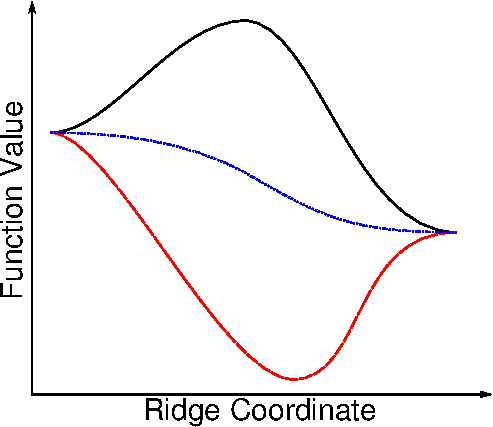
\includegraphics[width=0.45\linewidth]{bad-energy-profiles}
%    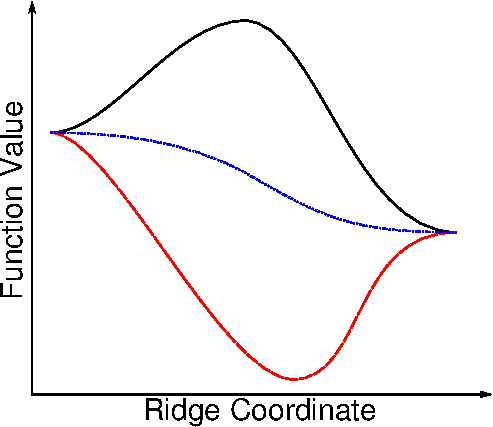
\includegraphics{bad-energy-profiles}
%    \parbox{0.85\linewidth}{
\caption{A schematic of some of some of the possible initial energy profiles of a ridge calculation.
A barrier (black, solid), a monotonic decrease (blue, dotted) and an inverted barrier (red, dashed).
Only the first is possible in NEB calculations.
}
\label{fig:bad-energy-profiles}
%}
%\end{center}
\end{SCfigure}

Since the end points of the ridge are not local minima, there is no intrinsic barrier separating them, as is the case for NEB calculations.
In fact, the initial profile can have any shape, including a monotonic one or even an inverted barrier, if it lies near a local minimum, which is \emph{not} unlikely, examples of which can be seen in \fref{fig:bad-energy-profiles}.
This means that the initial environment of the path is drastically different from that of the ridge.
To help bring the path nearer to the ridge, the full spring force was used.
Furthermore, the usage of the climbing image becomes questionable as the immobile end images may very well be the highest ones.
If using the climbing image from the outset is required, non-highest images must be used as the climbing image.
Images numbered $1$ and $N-1$ are partially restrained by the immobility of the endpoints, thus images even further in must be used, $2$ or $N-2$.

